\subsection{Número de coordinación}

De la misma manera que se definieron la distribuciones radiales de a pares parciales,
se pueden obtener los números de coordinación a un dado tipo de átomos. CN$_{ij}$
se corresponde con la cantidad de átomos vecinos de tipo $j$ para un átomo central
de tipo $i$ hasta una cierta distancia de corte. Para la elección de dicho valor 
se considera hasta el primer pico de la $g_{ij}(r)$ correspondiente. Debido a que 
en los materiales amorfos la primera y la segunda esfera de coordinación pueden 
llegar a estar superpuestas, el límite superior de integración no está definido 
unívocamente para todas las concentraciones consideradas ~\cite{lamparter1995}.
Para el número de coordinación promedio para átomos de Si vecinos de otros átomos 
de Si se calculó contando el número de dichos vecinos utilizando un radio de 
corte de 3 \AA. Lo mismo se realizó para Li-Li definiendo un radio de corte de 
4 \AA. Para el caso de Si-Li se utilizó el criterio de considerar como radio de 
corte el valor $r$ para el cual la $g(r)$ presenta un mínimo entre los dos picos
a primeros y segundo vecinos. Los resultados se muestran en la Figura 
\ref{fig:cn1}.
\begin{figure}[th]
    \centering
    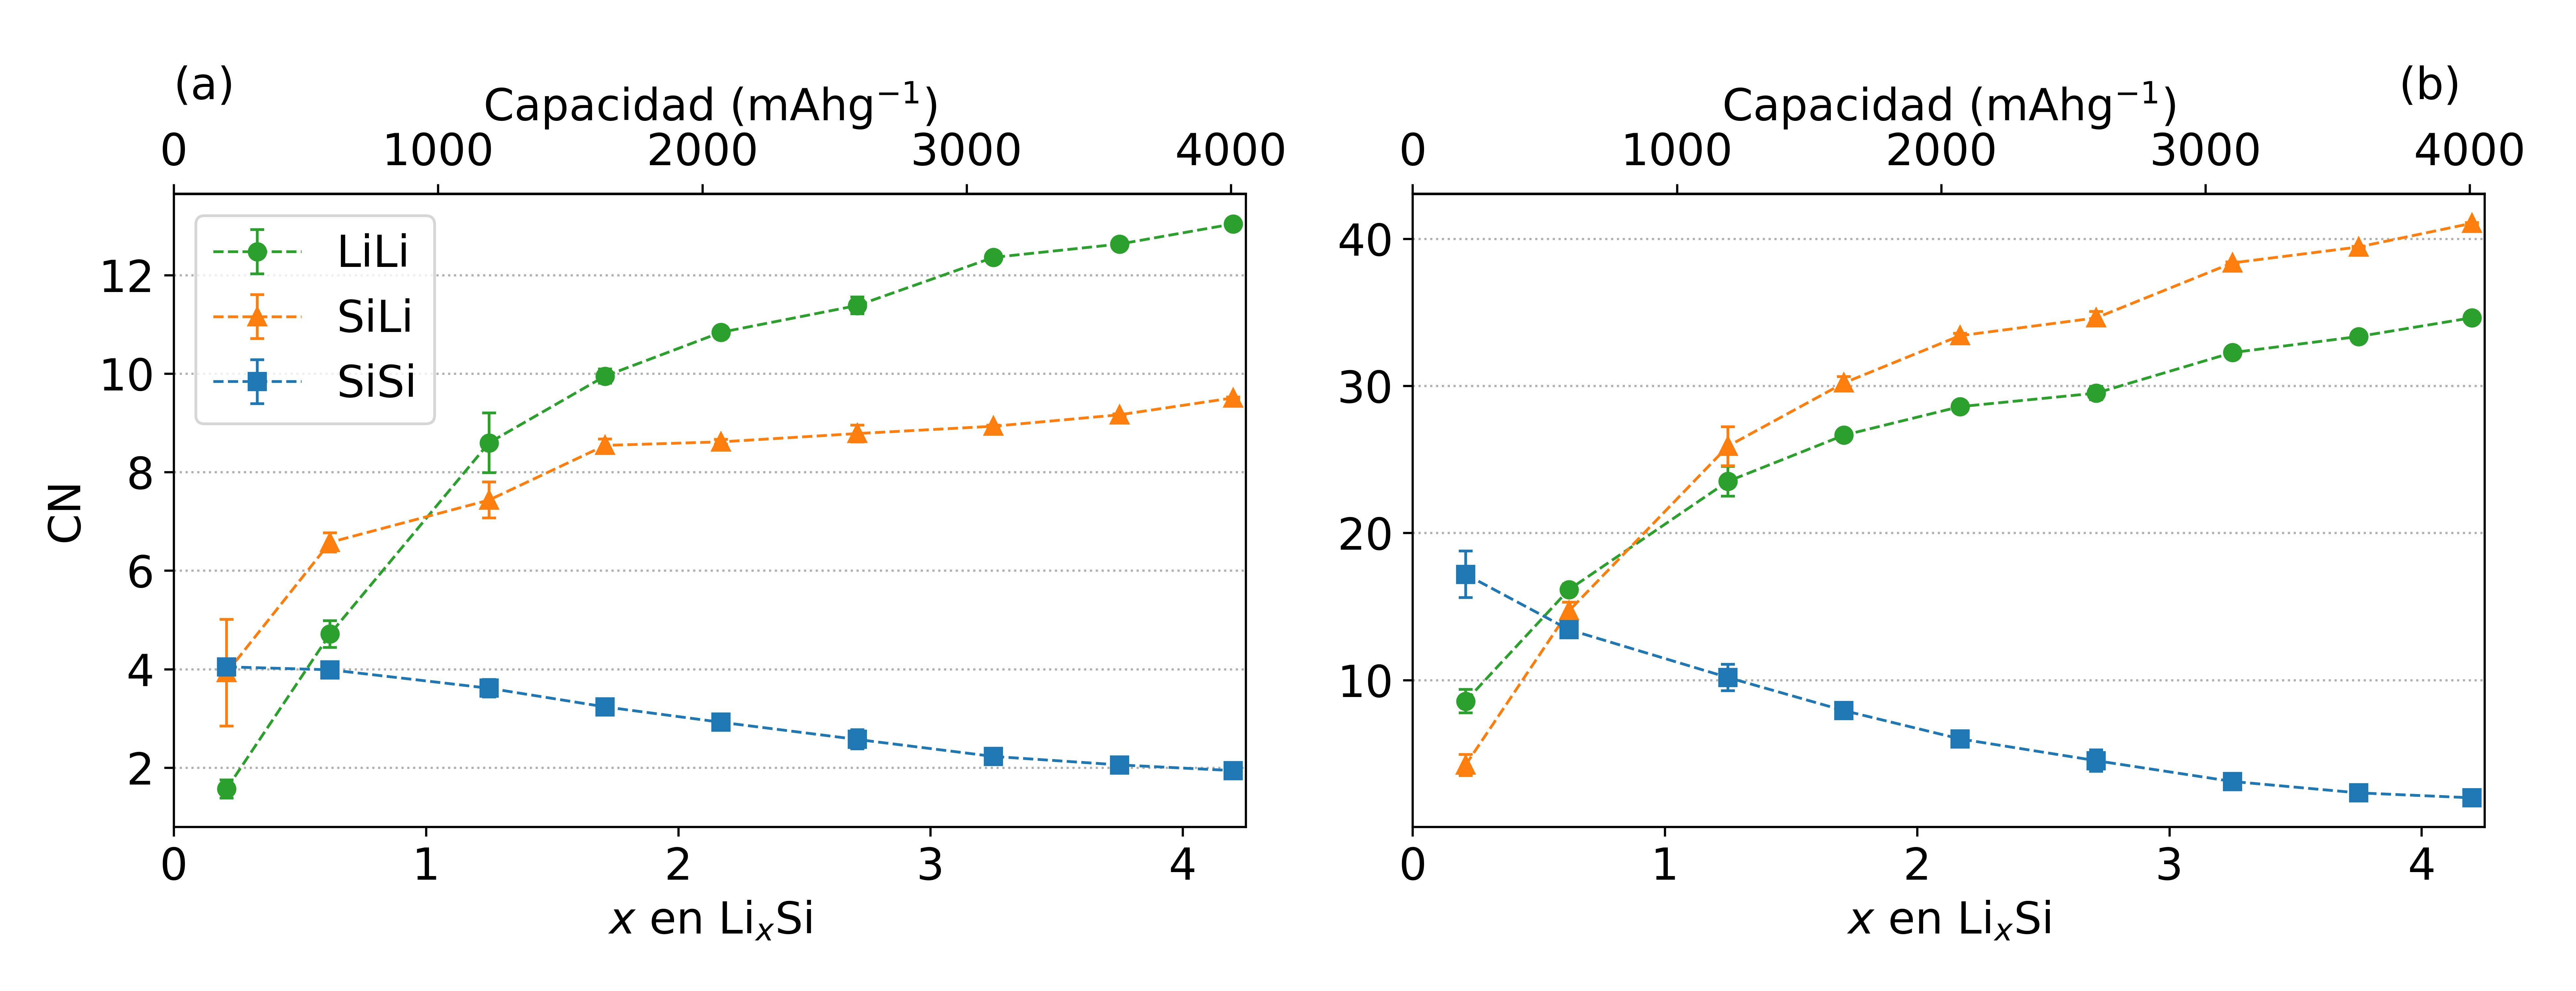
\includegraphics[width=0.8\textwidth]{Silicio/caracterizacion/resultados/cn/cn.png}
    \caption{Promedio del primer número de coordinación en función de la 
    concentración de litio para Li-Li, Si-Si y Si-Li. Como radio de corte se 
    utilizó la distancia posterior al primer pico de la RDF correspondiente. En 
    los casos en que no se aprecia la barra de error, es porque la misma es menor 
    que el tamaño de los puntos.}
    \label{fig:cn1}
\end{figure}

Para el caso del CN$_{\text{Si}-\text{Si}}$, se tiene que esta cantidad decrece de 4 a 2, a 
medida que la concentración de Li aumenta. Esto indica que a valores pequeños de 
$x$ la estructura de Si mantiene sus conexiones tetraédricas, mientras que para
valores grandes de $x$ el Si tiende a formar cadenas periódicas unidimensionales.
En la red de silicio amorfa, analizada con más detalle en la sección 
\ref{s:clusters}, una estructura 3-periódica se presenta para valores bajos de 
$x$, donde el CN se encuentra alrededor de 4. Luego, se alcanza una estructura 1-periódica 
para valores grandes de $x$, donde los enlaces Si-Si tienden a formar 
cadenas, que pueden verse para $x = 3.75$ donde se tiene $CN = 2.05$, por ejemplo.
El CN de Si-Li y Li-Li presenta valores pequeños para concentraciones 
bajas y aumenta monótonamente hasta alcanzar valores de 10 y 12, respectivamente, 
que se asemejan al valor de una estructura de empaquetamiento compacto.

\begin{figure}[th]
    \centering
    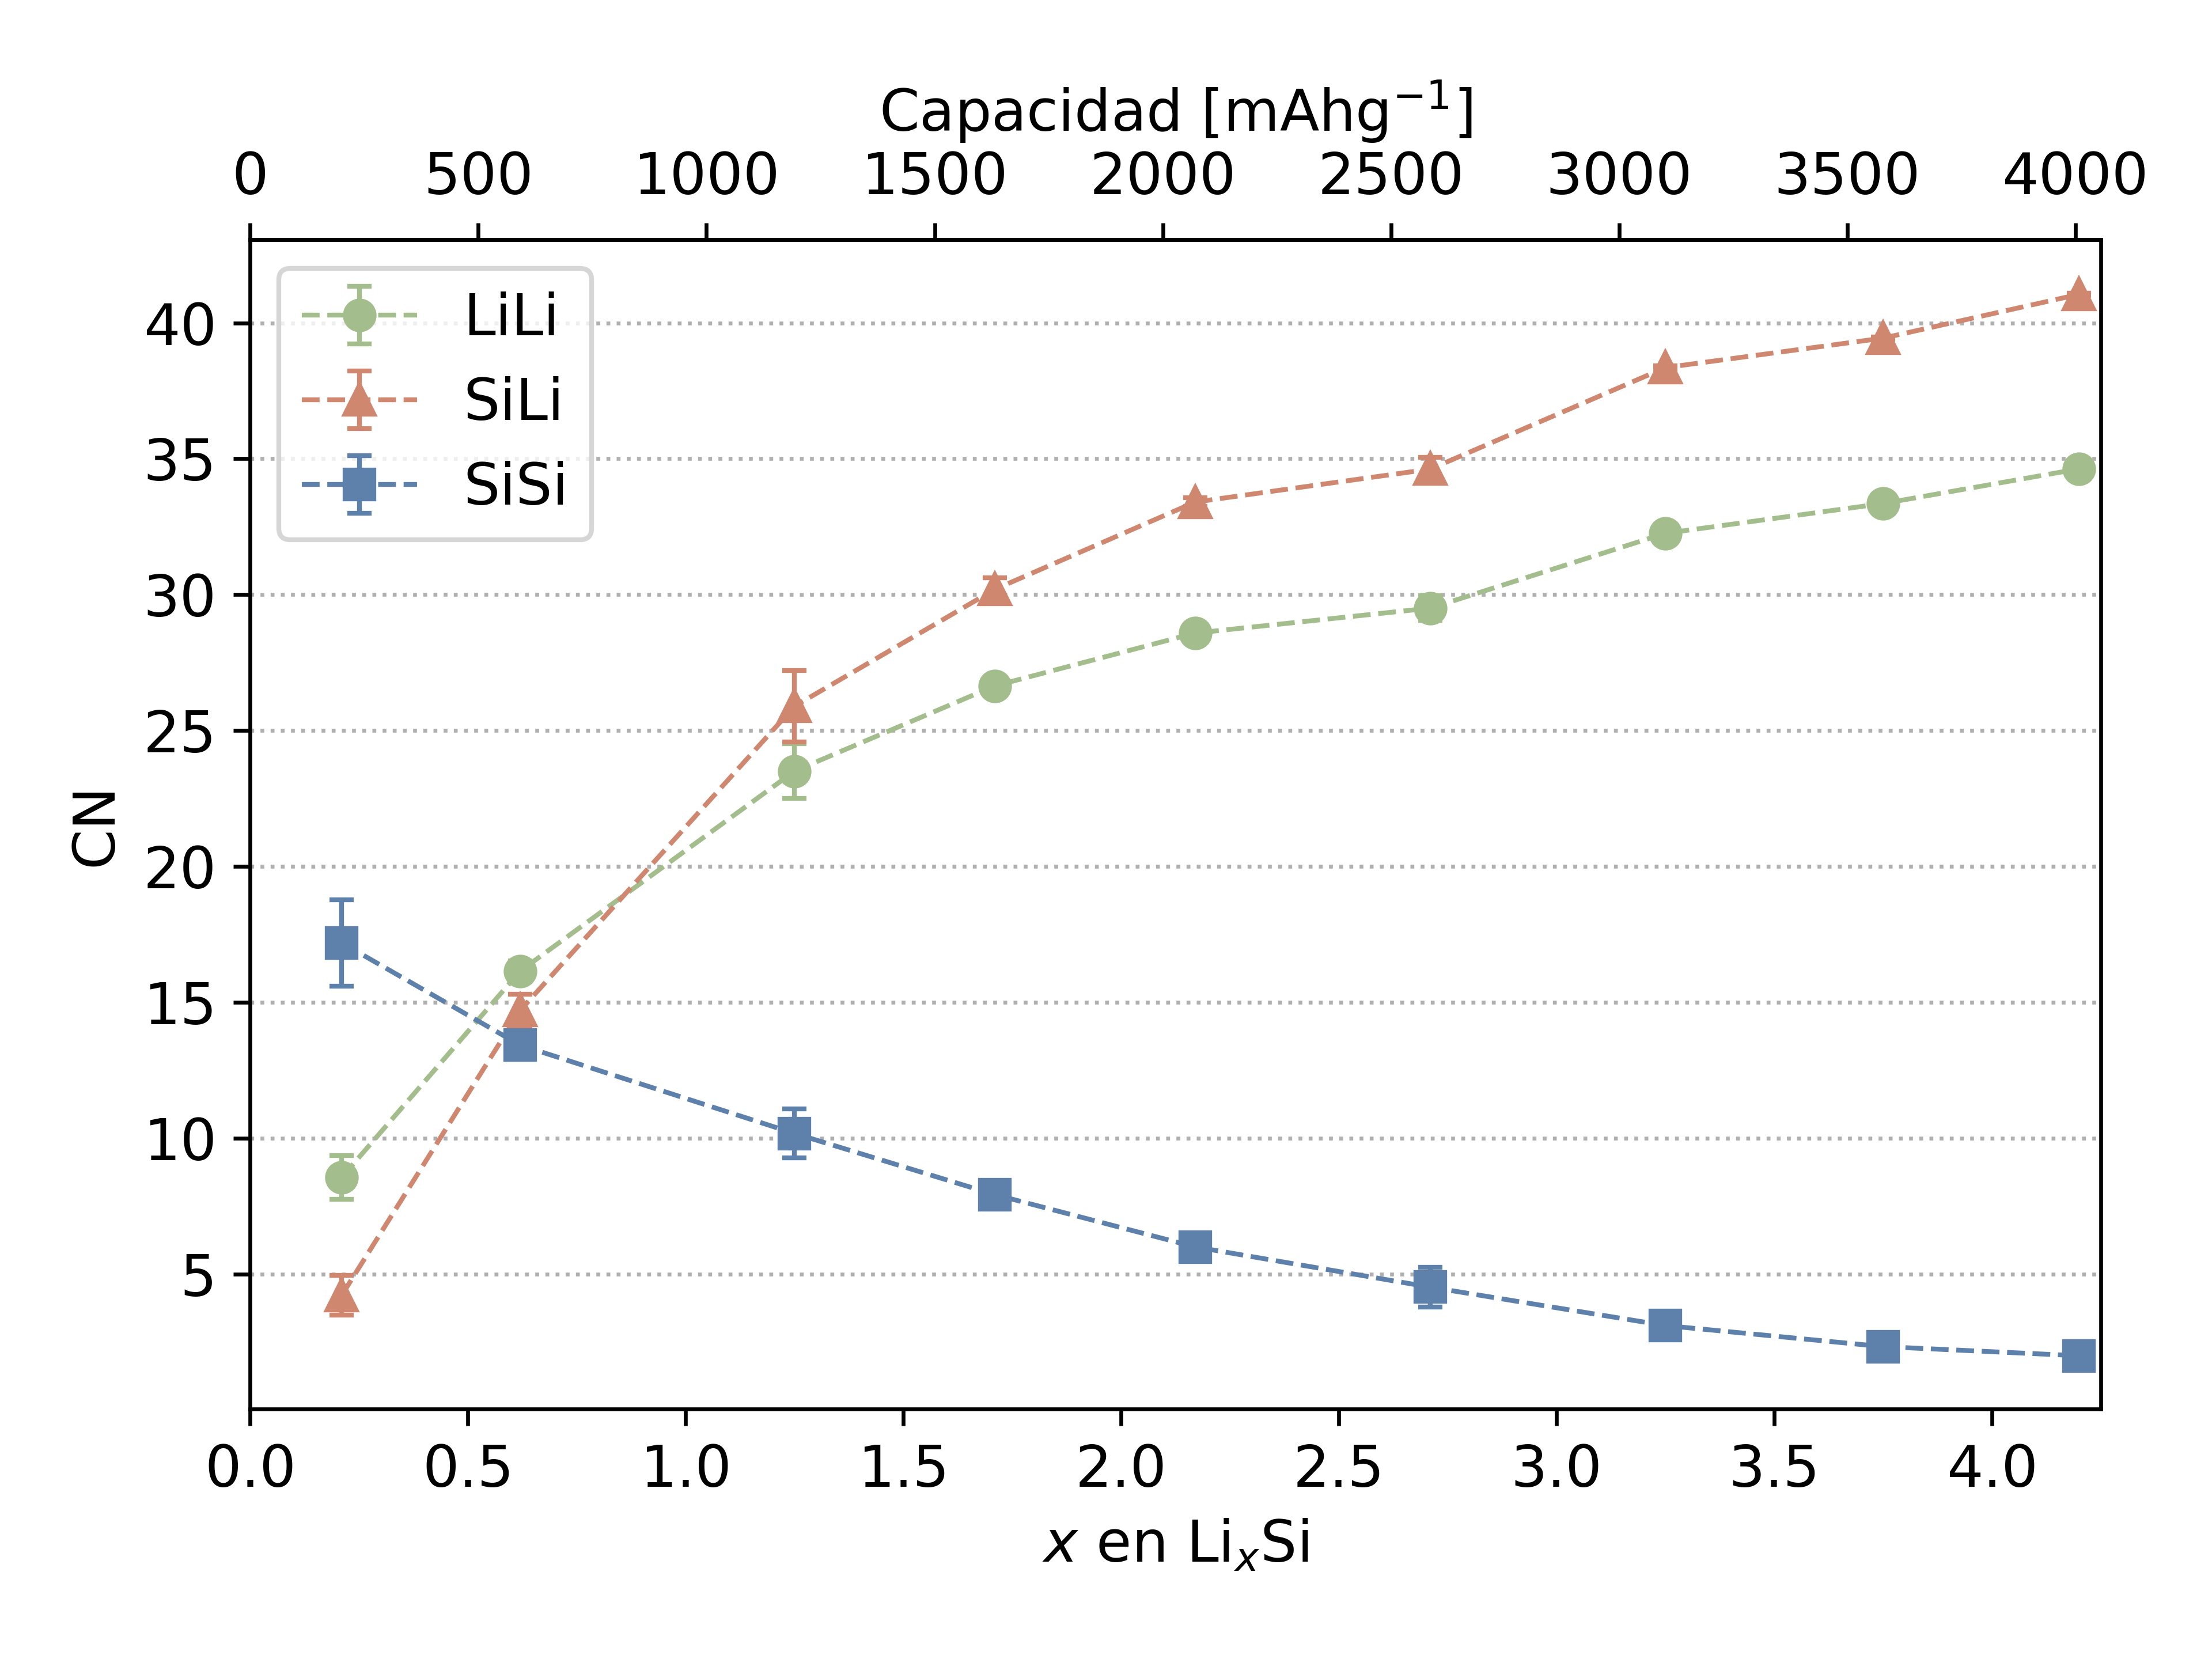
\includegraphics[width=0.8\textwidth]{Silicio/caracterizacion/resultados/cn/cn2.png}
    \caption{Promedio del segundo número de coordinación en función de la 
    concentración de litio para Li-Li, Si-Si y Si-Li. Para la elección de los 
    radios de corte que definen el cascarón en el cual se cuentan los vecinos,
    se consideró el segundo pico de la RDF correspondiente. En los casos que no 
    se aprecia la barra de error, es porque la misma es menor que el tamaño de 
    los puntos.}
    \label{fig:cn2}
\end{figure}
Los resultados para el segundo número de coordinación se presentan en la Figura 
\ref{fig:cn2}. Estos resultados se obtuvieron considerando un cascarón con un 
radio de corte interno y otro externo, elegidos de manera tal que incluyan el 
segundo pico de la RDF. La elección de dichos valores varió dependiendo del tipo
de átomos que se consideraron. En todos ellos se tomó como radio de corte interno 
el radio de corte del primero número de coordinación. Luego, para el radio de 
corte externo se utilizaron valores de 5.0 \AA\ para Si-Si y 6.0 \AA\ para Li-Li
y Si-Li.

Para los valores de CN$_{\text{Si}-\text{Si}}$ se observa un aumento para concentraciones bajas
de Li si se lo compara con el CN de primeros vecinos. Para valores mayores de $x$,
se puede ver como el valor de CN también tiende a 2, lo cual es coherente con la
formación de cadenas que se notó previamente. La tendencia cualitativa del segundo
CN para Li-Li y Si-Li es la misma a la observada en el primer CN, sólo que ahora
empieza en un valor cercano a 5 y tiende a 35 y 40, respectivamente. Este valor 
es mucho mayor que el que se tiene para los segundos vecinos en una estructura 
de empaquetamiento compacto, que es 6 para la estructura cristalina FCC. Incluso 
es mayor a la suma del segundo (6) y del tercer vecino (24) esperado para la red 
FCC.
